\chapter{Boosted Variational Bayesian Monte Carlo}

In this chapter, it is presented a modification of the Variational Bayesian Monte Carlo approach presented in Section \ref{vbmc_section}, using ideas of boosting presented in \ref{boostedvi_section}, along with some other minor modifications of the previous approach.

\section{Boosting Variational Bayesian Monte Carlo}

The idea underlying this approach is rather simple: instead of using a GP surrogate model for doing variational inference with mixtures of Gaussians as in \ref{vbmc_section}, use it for variational inference with the gradient boosting approach discussed in section \ref{boostedvi_section}.

To expand on this, consider again the algorithm in Figure \ref{vbalgorithm}. In line 5, the objective \eqref{relbogaussian} (here called \textit{$f$-step}) consists of three terms
\begin{displaymath}
 \begin{split}
 \text{RELBO}(\mu_i,\Sigma_i) = & \int \log(\gu(\theta)) \mathcal{N}(\theta|\mu,\Sigma) d\theta \\
 & - \int \log(q_{i-1}(\theta)) \mathcal{N}(\theta|\mu,\Sigma) d\theta \\
 & + \frac{\lambda}{4} \log |\Sigma|,
 \end{split}
\end{displaymath}
while in line 6, for the objective \eqref{boosting_objective_alpha} (here called \textit{$w$-step}), the gradient $\mathcal{L}'_i(w_i)$ consists of
\begin{displaymath}
\begin{split}
 \mathcal{L}'_i(w_i) = & \int \log (\gu(\theta)) f_{i}(\theta) \\ 
 & -\int \log(\gu(\theta)) q_{i-1}(\theta)\\
 & + \int \log((1-w_{i}) q_{i-1}(\theta) + w_{i} f_{i}(\theta)) (f_i(\theta) - q_{i-1}(\theta)) d\theta
\end{split}
\end{displaymath}

Then, in the same vein of the VBMC method, set a $GP(m,k)$ prior for $\log \gu$, and given evaluations $\mathcal{D}_0 = \{(x_i,f(x_i))\}_{i=1}^N$, substitute $\log \gu$ for $\Ev \log \gu_\mathcal{D}$. Since all the terms involving $\log \gu$ are expectations of either Gaussian distributions or mixture of Gaussian distributions, then one can approximate those by Bayesian Monte Carlo, as seen in \eqref{evvarbmcgaussian} and \eqref{bmcmixgaussians}, resulting in the maximization objective for the $f$-step:
\begin{equation}\label{relbo_vbmc}
\begin{split}
\text{RELBO}_\mathcal{D}(\mu_i,\Sigma_i) = & \int \Ev[\log \gu_\mathcal{D}(\theta)] \mathcal{N}(\theta|\mu_i,\Sigma_i) d\theta - \\ &\int \log(q_{i-1}(\theta)) \mathcal{N}(\theta|\mu_i,\Sigma_i) d\theta
+ \frac{\lambda}{4} \log |\Sigma_i|,
\end{split}
\end{equation}
and the maximization objective for the $w$-step
\begin{equation}\label{lalpha_vbmc}
\begin{split}
 \mathcal{L}_{i,\mathcal{D}}(w) = & \int \log \gu_\mathcal{D}(\theta)
 ((1-w_{i}) q_{i-1}(\theta) + w_{i} f_{i}(\theta)) d\theta - \\
 & \int \log ((1-w_{i}) q_{i-1}(\theta) + w_{i} f_{i}(\theta)) ((1-w_{i}) q_{i-1}(\theta) + w_{i} f_{i}(\theta)) d\theta \\
\end{split}
\end{equation}
with gradient
\begin{equation}
\begin{split}
\mathcal{L}'_{i,\mathcal{D}}(w) =& \int \Ev [\log \gu_\mathcal{D}(\theta)] f_{i}(\theta) - \int \Ev [\log \gu_\mathcal{D}(\theta)] q_{i-1}(\theta) + \\
& \int \log((1-w_{i}) q_{i-1}(\theta) + w_{i} f_{i}(\theta)) (f_i(\theta) - q_{i-1}(\theta)) d\theta,
\end{split}
\end{equation}
where
\begin{equation}
f_i(\theta) = \mathcal{N}(\theta|\mu_i,\Sigma_i), \quad q_{i-1}(\theta) = \sum_{k=0}^{i-1} w_k \mathcal{N}(\theta|\mu_k,\Sigma_k)
\end{equation}
The integrals not involving $\log \gu_\mathcal{D}$ can be easily approximated by the reparameterization trick, while $\log |\Sigma|$ is trivial to compute. This readily results in an algorithm for variational inference, given fixed evaluations points $\{x_n\}_{n=1}^N$, shown in Figure \ref{naivebvbmc}. Here it is named \textit{Naive Boosted Variational Bayesian Monte Carlo} (Naive BVBMC).
\begin{Algorithm}
\begin{algorithmic}[1]
	\Procedure{NaiveBVBMC}{$\log \gu,\mu_0$,$\Sigma_0$,$\{x\}_{n=1}^N$}
	\LineComment{$\mu_0,\Sigma_0$ the are initial boosting values}
	\For{$n=1,...,N$}
	\State $y_n := \log \gu(x_n)$
	\EndFor
	\State $\mathcal{D} := \{(x_n,y_n)\}_{i=1}^N$
	\State GPModel := PosteriorGP($m$,$k_{RBF}$,$\mathcal{D}$)
	\State GPModel.MaximizeLogLikelihood() \Comment{Using \eqref{loglikelihoodGP}}
	\State $\Ev[\log \gu_\mathcal{D}(\theta)]$ := GPModel.$m_\mathcal{D}$
	\State $w_0 := 1.0$
	\For{$t=1,...,T$}
	\LineComment{Using BMC and reparameterization}
	\State $\mu_{t},\Sigma_{t} := \argmax RELBO_\mathcal{D}(\mu_{t},\Sigma_{t})$
	\State $w_{t} := \argmax \mathcal{L}_{t,\mathcal{D}}(w_i)$ \Comment{Using $\mathcal{L}'_{t,\mathcal{D}}(w_t)$ for gradient descent}
	\For{$j=0,...,t-1$}
	\State $w_{j} \gets (1-w_t)w_j$
	\EndFor
	\EndFor
	\State \Return $\{(\mu_t,\Sigma_t,w_t)\}_{t=1}^T$
	\EndProcedure
\end{algorithmic}
\caption{\label{naivebvbmc} Naive boosted variational bayesian monte carlo}
\end{Algorithm}
\subsection{Practical issues}
The algorithm in Figure \ref{naivebvbmc} run into some practical issues, described below, that requires fixes of an heuristic nature. Here we present the heuristics that were used to make the algorithm stable. The resulting algorithm in found in \ref{bvbmcalgorithm}.

\subsubsection{RELBO stabilization}
By letting $r_\mathcal{D}(\theta) := \exp \Ev \log_\mathcal{D}(\theta)$, consider again the maximization objective \eqref{relbo_vbmc}, rewritten as
\begin{equation}
 \text{RELBO}_\mathcal{D}(\mu_i,\Sigma_i) = \int \log \left(\frac{r_\mathcal{D}(\theta)}{q_{i-1}(\theta)} \right) \mathcal{N}(\theta;\mu_i,\Sigma_i) d \theta + \log |\Sigma_i|.
\end{equation}
Assume $\Sigma_i$ fixed for now, so that the only term being optimized is $\mu_i$. Then, what the maximizer "wants" to do is set $\mu_i$ in a place that $\mathcal{N}(\theta;\mu_i,\Sigma_i)$ allocates probability mass where $\log r_\mathcal{D}(\theta)/q_{i-1}(\theta)$ is large. Now, consider the tail behavior of this quantity. We have that $q_{i-1}(\theta) \approx C_1 \exp(-||A_1(\theta-c_1)||_2^2)$ on the tail, while either $r_\mathcal{D}(\theta) \approx \exp(-C)$, if $m(\theta) = -C$, or $r_\mathcal{D}(\theta) \approx \exp(-||A_2(\theta-c_2)||_2^2)$, in case of $m(\theta) = -||A_2(\theta-c_2)||_2^2$. In the first case, then $\log r_\mathcal{D}(\theta)/q_{i-1}(\theta) \to \infty$ as $\theta \to \infty$, while in the second case, whether this happens depends on the relation between $A_1$ and $A_2$. However, if $\log r_\mathcal{D}(\theta)/q_{i-1}(\theta) \to \infty$ as $\theta \to \infty$, then the maximizer will try to get $\mu_i$ to $\infty$, thus resulting in bad proposals, that ends up with negligible weights $w_i$.

One approach to deal with this problem is to replace the term $\log r_\mathcal{D}/q_{i-1}(\theta)$ by $\log r_\mathcal{D}/(q_{i-1}(\theta)+\delta_D)$, where $\delta_D$ is a small positive constant. This approach is similar to the one in \cite{Guo_2016}, where a regularizer is added to both numerator and denominator, although it is done in the approximate heuristic proposed there. Thus, the $f$-step maximization objective becomes

\begin{equation}
\text{RELBO}^{\delta_D}_\mathcal{D}(\mu_i,\Sigma_i) = \int \log \left(\frac{r_\mathcal{D}(\theta)}{q_{i-1}(\theta)+\delta_D} \right) \mathcal{N}(\theta;\mu_i,\Sigma_i) d \theta + \log |\Sigma_i|.
\end{equation}

In the current work, $\delta_D = e^{-20}$ by default.

\subsubsection{Output scaling}\label{outputscaling}
One issue that arises with unnormalized log-densities is that one has no control on its scale. Fortunately, scaling the output can be done easily. Given data $\mathcal{D} = \{(x_i,y_i)\}_{i=1}^N$, suppose one makes a linear transformation $\tilde{y}_i = \frac{y_i-b}{a}$, and, letting $\tilde{\mathcal{D}} = \{x_i,\tilde{y}_i\}$, consider the GP posterior $f_{\tilde{\mathcal{D}}} \sim GP(m_{\tilde{\mathcal{D}}},k_{\tilde{\mathcal{D}}})$. Then, the random function $a f_{\tilde{\mathcal{D}}} + b$ is GP distributed, and
\begin{equation}
\int (a f_{\tilde{\mathcal{D}}} + b)(x) p(x) dx 
\end{equation}
is a GP random variable, with
\begin{equation}
\Ev \left[\int (a f_{\tilde{\mathcal{D}}} + b)(x) p(x) dx \right] = a \Ev \left[ \int f_{\tilde{\mathcal{D}}}(x) p(x) dx \right] + b,
\end{equation}
and variance 
\begin{equation}
\Var \left(\int (a f_{\tilde{\mathcal{D}}} + b)(x) p(x) dx \right) = a^2 \Var \left( \int f_{\tilde{\mathcal{D}}}(x) p(x) dx \right).
\end{equation}
This implies that one can do BMC, hence also VBMC and BVBMC using affinely scaled output variables, without difficulty.

Two heuristic for scaling were implemented, the \textit{normalize} heuristic, given by
\begin{itemize}
	\item Letting $y_i = \log g(x_i)$, calculating the sample mean $m_y = \frac{1}{N} \sum_{i=1}^N y_i$ and the (unbiased) sample standard deviation $\sigma_y = \sqrt{\frac{1}{N-1} \sum_{i=1}^N (y_i-m_y)}$.
	\item Transforming the output $\tilde{y}_i = (y_i-m_y)/\sigma_y$.
	\item Train a GP (along with hyperparameters) on $\tilde{\mathcal{D}} = \{x_i,\tilde{y}_i\}_{i=1}^N$.
	\item Substituting, when needed, $\log g_\mathcal{D}(x)$ (and their integrals) for $\sigma_y \log g_\mathcal{\tilde{D}}(x) + \mu_y$
\end{itemize}
and the \textit{zeromax} heuristic, where
\begin{itemize}
	\item Letting $y_i = \log g(x_i)$, calculating the sample maximum $m_y = \max\{y_i\}_{i=1}^N$ and making $\sigma_y = 1$.
	\item Do the other steps as in \textit{normalize} heuristic.
\end{itemize}
In toy problems presented in the next section, both heuristics worked well, but for more complex problems the \textit{zeromax} heuristic was found to be more stable.

\subsubsection{Component initialization}
A question that still wasn't addressed is on how to choose the first boosting component. Two options were tested:
\begin{itemize}
	\item Initializing the first mixture component with zero mean and a large covariance.
	\item Choosing the first component by maximizing the ELBO between the component and GP surrogate.
\end{itemize}
In general, the second method was chosen in this work, although performance in both cases was comparable.

\subsubsection{Component pruning}
When running the BVBMC algorithm, many mixture components may end up with negligible weights. This may both increase the computational cost of the algorithm, and hinder the performance of joint parameter updating (explained in \ref{jointparameterupdating}). In order to diminish this problem, an weight threshold $\beta$ may be established, so that, if $(w_1,\ldots,w_N)$ are the current mixture weights, every $i$-th mixture components with $w_i < \beta$ is removed, with the remainder weights being renormalized to one. This pruning may be done either every iteration, or only when doing joint parameter updating (for which pruning proved necessary).

\subsubsection{Mean functions}\label{meansection}
As discussed in Section \ref{quadmeanfnsection}, one option for the mean function set $m(\theta) = m_Q(\theta;l,c)$ as in \eqref{vbmc_quadratic_mean}. However, one issue that arose in this work is that optimizing $l,c$ by maximizing the log-likelihood often resulted in very large values (in absolute value) for $l$ and $c$, destabilizing the algorithm.

In this light, a different approach for the mean is proposed, by letting
\begin{equation}
m_F(\theta) = C
\end{equation}
where $C$ is a large negative constant, that is \textit{fixed before hyperparameter optimization}. Strictly speaking, in this case $\exp \Ev[\log \gu_\mathcal{D}(\theta)]$ is not anymore a probability distribution. However, if $C$ is sufficiently low, it resembles a probability distribution enough so that the algorithm works well in practice.

Since $C$ is not set by optimizing the log-likelihood, one must decide on how to set it. If the data was scaled beforehand using \textit{zeromax}, some good options that worked well in practice were $C = -10,-20,-30$. For scaling using \textit{normalize}, the following way to set $C$ is proposed:
\begin{equation}
C = \tilde{y}_{\min} - K_{C}(\tilde{y}_{\max} - \tilde{y}_{\min}),
\end{equation}
where $\tilde{y}_{\max}$ and $\tilde{y}_{\min}$ are the maximum and minimum of the normalized output values, and $K_C > 0$ is a constant. In this work, $K_C = 1$ was found to be a good choice.

\subsubsection{Periodic joint parameter updating}\label{jointparameterupdating}
Sometimes, boosting may get \enquote{stuck}, in the sense that the variational proposal takes too long to improve. In that case, one may desire to periodically update all variational parameters in the sense of the original VBMC algorithm. However, since this optimization is expensive, it should be used sparsely, for example every 10 boosting steps, or every 3 steps when boosting does not show improvement, when checking the ELBO.

\subsubsection{Other kernel functions}
As discussed in Section \ref{tensorprodbmc}, tensor product of one-dimensional kernels can be easily integrated with Bayesian Monte Carlo with diagonal covariance Gaussian distributions. In this light, by letting $k_{\text{Matern},\nu}(|x-x'|;l)$ be the 1-d Matérn kernel, the product of Matérn kernels is defined
\begin{equation}
 k_{\text{PMat},\nu}(x,x';\theta,l) = \theta \prod_{d=1}^D k_{\text{Matern},\nu}(|x_i-x_i'|;l_d).
\end{equation}
It must be noted that the product of Matérn kernels is \text{not} the Matérn kernel for $d > 1$, although it is a stationary kernel.

In experiments, the product of Matérn kernels tended to be more stable than the squared exponential kernel, particularly for $\nu = 1/2,3/2$, although for $\nu = 5/2$ the cases where it became unstable were rare. This may be due to the fact that the squared exponential kernels assumes far too much smoothness in its defined GP, hence estimating large oscillations outside the domain of interest, resulting in spurious multimodality.

\subsection{Other acquisition functions for active evaluation}
One problem that may arises in prospective prediction is that the term $\exp(m_\mathcal{D}(\theta_{N+1}))$ may become unstable for high values. Hence, one change proposed in this work is to substitute $\exp$ for the function $\text{softplus}(x) = \log(1+\exp(x))$, resulting in the \textit{soft prospective prediction}
\begin{equation}\label{soft_prospective_vbmc}
\alpha^\mathcal{D}_{PP}(\theta_{N+1}) = k_\mathcal{D}(\theta_{N+1},\theta_{N+1}) \text{softplus}(m_\mathcal{D}(\theta_{N+1}))q_k(\theta_{N+1};\lambda)^2.
\end{equation}
Another option is to disregard the current proposal altogether, and instead noticing that, ideally, the proposal is going to approximate the unnormalized posterior $\gu = \exp \log \gu$. Hence, one can take as an inspiration the warping approach in Section \ref{positivebmc} and use the \textit{moment-matched log transform} objective 
\begin{equation}\label{mmlt_vbmc}
\alpha^m_{MMLT}(x_{m+1}) = e^{2 m_\mathcal{D}(x) + k_\mathcal{D}(x,x)} \left(e^{k_\mathcal{D}(x,x')}-1\right).
\end{equation} 
Finally, one can adapt the uncertainty sampling approach to the warped approach, resulting in the \textit{prospective moment-matched log transform} objective
\begin{equation}\label{mmltprop_vbmc}
\alpha^m_{MMLT_P}(x_{m+1}) = e^{2 m_\mathcal{D}(x) + k_\mathcal{D}(x,x)} \left(e^{k_\mathcal{D}(x,x')}-1\right)q_k(\theta_{N+1};\lambda)^2.
\end{equation}
In general, the best performing acquisition functions were \eqref{prospective_vbmc} and \eqref{mmlt_vbmc}, and best results were obtained alternating between the two, either cyclically or randomly.

\begin{Algorithm}
\begin{algorithmic}[1]
	\Procedure{BoostedVBMC$_0$}{$\log \gu,\mu_0$,$\Sigma_0$,$\{x\}_{n=1}^N$,$\delta_D$}
	\LineComment{$\mu_0,\Sigma_0$ the are initial boosting values}
	\For{$n=1,...,N$}
	\State $y_n := \log \gu(x_n)$
	\EndFor
	\State $\mathcal{D}_0 := \{(x_n,y_n)\}_{i=1}^N$
	\State Make $\tilde{\mathcal{D}}$ from $\mathcal{D}$. Hold $m_y$ and $\sigma_y$. \Comment{Section \ref{outputscaling}}
	\State GPModel := PosteriorGP($m$,$k$,$\mathcal{D}$)
	\State GPModel.MaximizeLogLikelihood() \Comment{Using \eqref{loglikelihoodGP}}
	\State $\Ev[\log \gu_\mathcal{D}(\theta)]$ := GPModel.$m_\mathcal{D}$
	\State $\alpha_0 := 1.0$
	\State $(\mu_0,\Sigma_0)\ \gets \argmax \mathcal{L}_\mathcal{D}(\lambda)$ \Comment{Section \ref{outputscaling}}
	\For{$t=1,...,T$}
		\State $x' := \argmax \alpha^m(x)$ \Comment{Some acquisition function}
		\State $y' = \log \gu(x')$
		\State $\tilde{y}' = \frac{y - m_y}{\sigma_y}$
		\State $\tilde{\mathcal{D}} \gets \tilde{\mathcal{D}} \cup \{(x',\tilde{y}')\}$
		\LineComment{Using BMC and reparameterization}
		\State $\mu_{t},\Sigma_{t} := \argmax RELBO^{\delta_D}_\mathcal{D}(\mu_{t},\Sigma_{t})$
		\State $w_{t} := \argmax \mathcal{L}_{t,\mathcal{D}}(w_i)$ \Comment{Using $\mathcal{L}'_{t,\mathcal{D}}(w_t)$ for gradient descent}
		\For{$j=0,...,t-1$}
			\State $w_{j} \gets (1-w_t)w_j$
		\EndFor
		\If{conditions met}
			\State $\lambda = \{(\mu_j,\Sigma_j,w_j)\}_{j=1}^t \gets \argmax \mathcal{L}_\mathcal{D}(\lambda)$ \Comment{Section \ref{jointparameterupdating}}
		\EndIf
	\EndFor
	\State \Return $\{(\mu_t,\Sigma_t,w_t)\}_{t=1}^T$
	\EndProcedure
	\caption{\label{bvbmcalgorithm}Boosted Variational Bayesian Monte Carlo}
\end{algorithmic}
\end{Algorithm}

\section{Implementation}
The algorithm was implemented in Python, mainly using the PyTorch package \cite{Paszke_2017}. The reason for using PyTorch is that it combines strong automatic differentiation capabilities, allowing to avoid computing derivatives by hand, with easy usability when compared to other packages with similar strenghts such as TensorFlow. Since derivatives are necessary for the many inner optimization procedures in the algorithm,automatic differentiation greatly facilitated development. 

Code can be found in \url{https://github.com/DFNaiff/BVBMC}. An example usage of the package is shown in Figure \ref{bvbmcpackexample}, with associated densities shown in \ref{bvbmcpackfigs}. \footnote{The author intends to change the package name used in development, \textit{variational\_boosting\_bmc}, to something akin to \textit{bvbmc}, but the change wasn't made at this document writing.}

\begin{figure}\label{bvbmcpackexample}
	\begin{lstlisting}
	#Import necessary packages
	import torch #PyTorch package
	from variational_boosting_bmc import VariationalBoosting #BVBMC package
	
	#Approximating unnormalized 2-d Cauchy
	def logjoint(theta):
		return torch.sum(-torch.log(1+theta**2))
	
	#Set up parameters
	dim=2 #Dimension of problem
	samples = torch.randn(20,dim) #Initial samples
	mu0 = torch.zeros(dim) #Initial mean
	cov0 = 20.0*torch.ones(dim) #Initial covariance
	acquisition = "prospective" #Acquisition function
	
	#Initialize algorithm
	vb = VariationalBoosting(dim,logjoint,samples,mu0,cov0)
	vb.optimize_bmc_model() #Optimize GP model
	vb.update_full() #Fit first component
	
	#Training loop
	for i in range(100):
		_ = vb.update() #Choose new boosting component
		vb.update_bmcmodel(acquisition=acquisition) #Choose new evaluation
		vb.cutweights(1e-3) #Weights prunning
		if ((i+1)%20) == 0:
			vb.update_full(cutoff=1e-3) #Joint parameter updating
	
	vb.save_distrib("finaldistrib") #Save distribution
	\end{lstlisting}
	\caption[Usage of the BVBMC Python package.]{\label{bvbmcpackexample}Usage of the BVBMC Python package, approximating a product of Cauchy distributions.}
\end{figure}

\subsection{Backpropagation}
Usually, in an algorithm with so many optimization steps, one would either have to worry about carefully keeping control of gradients, or resort to gradient free optimization. However, backpropagation \cite{Goodfellow_2016}, a technique from the class of automatic differentiation algorithms, allows the computer to provide arbitrary derivatives of functions, provided the forward history of the function is tracked.

A formal discussion on backpropagation is beyond the scope of this work. A good reference can be found in \cite{Goodfellow_2016}. Greatly simplifying, backpropagation hinges on the fact that almost every function in a computer comes from composition, so the chain rule can be applied. So, if the forward history of the composition is stored in a suitable data structure (a \textit{computational graph}), then, given the derivatives of those unit compositions, chain rule can be applied to get any derivative, without ever needing for then to being calculated by hand.

Backpropagation is ubiquitous in deep learning , and almost all packages dealing with neural networks implement some form of it. In fact, most of then are backpropagation packages, in which neural networks are build on top of it. Some of the most popular are Theano \cite{Theano_2016}, TensorFlow \cite{Abadi_2015} and PyTorch \cite{Paszke_2017}. Of those, PyTorch is the one with easiest usability, so it was chosen to implement the BVBMC package.

The usefulness of backpropagation and their related packages in general escapes the community outside deep learning. An important exception is in development of probability programming languages (PPL), whose many are built on top of deep learning packages, as in PyMC3 \cite{Salvatier_2016}, Edward \cite{Tran_2016} and Pyro \cite{Bingham_2018}, built on top of Theano, TensorFlow and PyTorch, respectively.

\begin{figure}
	\centering
	\subfloat[True density]{\label{fig11a}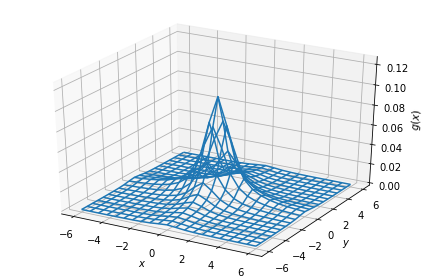
\includegraphics[width=0.4\linewidth]
		{figs/examplebvbmctrue.png}}
	\subfloat[Estimated density]{\label{fig11b}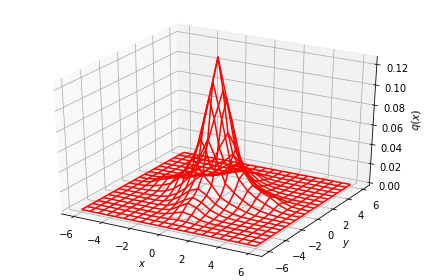
\includegraphics[width=0.4\linewidth]
	{figs/examplebvbmcestimated.png}}

	\caption[\label{bvbmcpackfigs}True density and estimated density found by running code in Figure \ref{bvbmcpackexample}]{\label{bvbmcpackfigs}True density (left) and estimated density (right), found by running code in Figure \ref{bvbmcpackexample}. Generating code can be found in \url{https://github.com/DFNaiff/Dissertation/blob/master/illustrations_dissertation/examplebvbmc.py}.}
\end{figure}
